\newpage

\section{Systémové požadavky}
Aplikace ke svému běhu potřebuje počítač nainstalovaným operačním systémem
\textbf{GNU/Linux}. Dále vyžaduje funkční \textbf{webovou kameru}. Processor
alespoň \textbf{1.6GHz} (v této konfiguraci sice není ovládání příliš plynulé,
ale je použitelné).

\section{Softwarové závislosti}
Aplikace využívá některé knihovny a frameworky, které je potřeba mít
nainstalované v systému, aby bylo možné zkompilovat a spustit.

\begin{itemize}
    \item \textbf{Qt Framework 4.8}\\
    \url{http://qt.nokia.com}
    \item \textbf{Boost 1.49.0}\\
    \url{http://www.boost.org}
    \item \textbf{Xlib} \\
    \url{http://www.x.org}
    \item \textbf{libv4l2} \\
    \url{http://linuxtv.org}
\end{itemize}

\section{Sestavení a instalace}
Pro sestavení aplikace je potřeba mít tyto nástroje:

\begin{itemize}
    \item \textbf{Make} \\
    \url{http://www.gnu.org/software/make/}
    \item \textbf{pkg-config} \\
    \url{http://www.freedesktop.org/wiki/Software/pkg-config}
    \item \textbf{GCC 4.7.0} (byli použity konstrukce ze standardu C++11) \\
    \url{http://gcc.gnu.org/}
\end{itemize}

\bigskip\noindent
Dále zmiňované projekty naleznete na přiloženém CD. Před sestavením, je třeba
projekty zkopírovat mimo CD do nějaké zapisovatelné složky.

\bigskip\noindent
Nejprve je potřeba sestavit a nainstalovat \textbf{FakeInput} a
\textbf{Gecon Framework}.

Posloupnost příkazů příkazové řádky pro sestavení je následující:

\begin{quote}
\texttt{> cd <složka-projektu>}\\
\texttt{> make config=release}
\end{quote}

FakeInput a Gecon Framework je třeba nainstalovat aby byli vyhledatelné v
systému. Buď se nainstalují přímo do standardních instalačních cest v systému,
nebo je možné využít \uv{vývojářské} instalace, která nainstaluje soubory v
rámci projektové složky.

Standardní instalace:
\begin{quote}
\texttt{> make install intall\_prefix=<prefix-pro-instalaci>}
\end{quote}

\uv{Vývojářská} instalace:
\begin{quote}
\texttt{> make dev-install}
\end{quote}

Pokud se projekty nainstalují pomocí \uv{vývojářské} instalace nebo do
nestandardní cesty, je třeba přidat instalační cesty do proměnných prostředí:

\begin{quote}
\small
\texttt{> LD\_LIBRARY\_PATH=\$LD\_LIBRARY\_PATH:<prefix-FakeInput>/lib}\\
\texttt{> LD\_LIBRARY\_PATH=\$LD\_LIBRARY\_PATH:<prefix-GeconFramework>/lib}\\
\texttt{> export LD\_LIBRARY\_PATH}
\end{quote}
\begin{quote}
\small
\texttt{>
    PKG\_CONFIG\_PATH=\$PKG\_CONFIG\_PATH:<prefix-FakeInput>/lib/pkgconfig}\\
\texttt{>
    PKG\_CONFIG\_PATH=\$PKG\_CONFIG\_PATH:<prefix-GeconFramework>/lib/pkgconfig}\\
\texttt{> export PKG\_CONFIG\_PATH}
\end{quote}

\texttt{<prefix-FakeInput>} a \texttt{<prefix-GeconFramework>} jsou prefix
nastavené při instalaci, v případě \uv{vývojářské} instalace jsou to složky
projektů.

\bigskip
Nyní je možné sestavit \textbf{Gecon PC}.
\begin{quote}
\texttt{> cd <složka-GeconPC>}\\
\texttt{> make config=release}
\end{quote}

Aplikaci spustíme pomocí \texttt{make run}.

\section{Práce s aplikací}
V této sekci popíšeme, jak se pracuje s aplikací. Hlavní okno programu vypadá
jako na obrázku 1.

\begin{figure}[h]
\centering
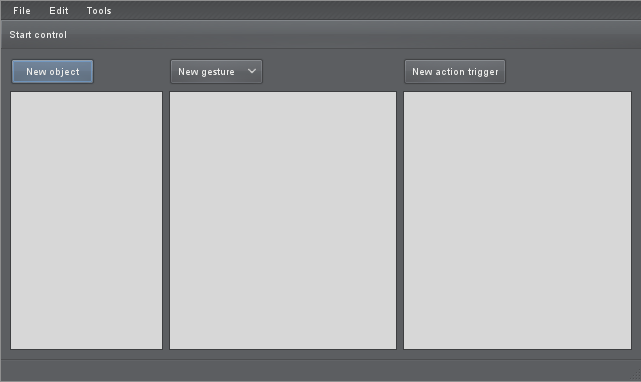
\includegraphics[width=\textwidth]{mainwindow.png}
\caption{Hlavní okno}
\end{figure}

Je rozděleno na tři části: část pro objekty (vlevo), část pro gesta
(uprostřed) a část pro spoštěče akcí (vpravo).

Panel pod nabídkou menu obsahuje tlačíto \emph{Start control}, které spouští
kontrolní cyklus ovládání. Před spuštěním je ale potřeba přidat objekty, gesta
a spouštěče akcí.

\subsection{Nastavení webové kamery}
Pokud je k počítači připojeno více webových kamer, tu správnou si vyberete
pomocí dialogu nastavení \emph{Settings}. Nachází se v nabídce \emph{Edit}.

\begin{figure}[h]
\centering
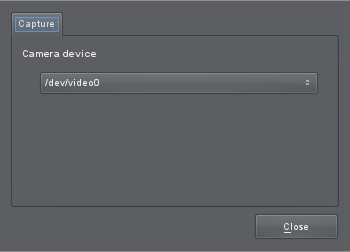
\includegraphics[width=0.7\textwidth]{settings.png}
\caption{Výběr webové kamery}
\end{figure}

Pokud nejsou k dispozici žádná zařízení, aplikace o tom dá vědět varovnou
hláškou. V tom případě bude aplikace dále fungovat, jen nebude funkční vše co
pracuje se snímky z kamery (tedy práce s objekty, s pohybovými gesty a samotné
ovládání).

\subsection{Práce s objekty}
Nový objekt se přidává před dialog, který se aktivuje kliknutím na tlačítko
\emph{New object}. Dialog je vyobrazen na obrázku 2. Uprostřed je zobrazeno
video snímané kamerou. Pro získání barvy objektu, je třeba umístit objekt, tak
aby byl vidět v záběru a po té na něj kliknout. Detekovaný objekt pak bude
vyznačen oblastí vyplněnou modrými tečkami a zeleným konvexním obalem a
červeným opsaným obdélníkem.

Pokud se bude vyznačena jiná oblast, než jste očekávali, zkuste kliknout do
různým míst v objektu. Pokud ani to nepomůže, je buď špatné osvětlení, barva
objektu je málo výrazná nebo se v pozdaní nachází příliš podobný objekt.

\begin{figure}[h]
\centering
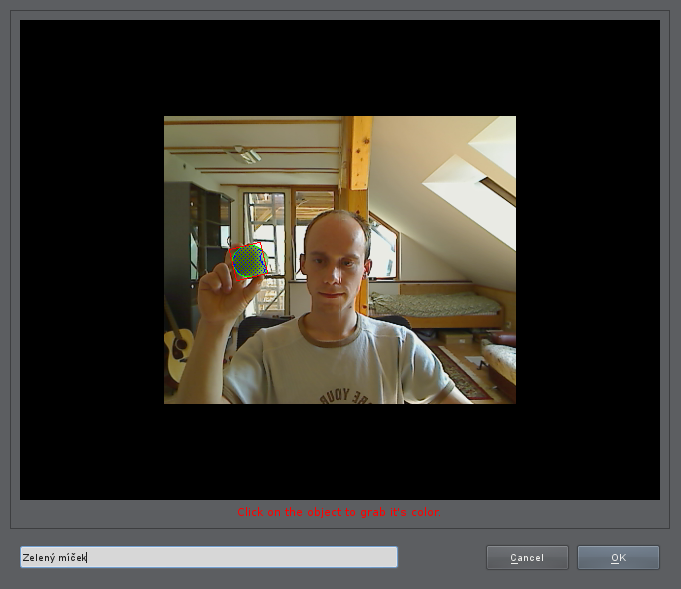
\includegraphics[width=\textwidth]{newobject.png}
\caption{Dialog pro přidání nového objektu}
\end{figure}

Objekty vybírejte s pokud možno co nejsytější barvou. Osvětlení je vhodné
čelní, nikoli však přímé. Jako vhodné se ukálazo sedět proti oknu (samozřejmě
ne s přímým sluncem) nebo sedět proti stěně a namířit na ni rozsvícenou
lampičku.

Po vyznačení objektu s ním zkuste pohybovat, natáčet ho, oddalovat i
přibližovat, abyste zjistili, zda bude správně vyznačen i v jiných místech
záběru. Také zkuste objektem vyjet mimo záběr, ideální je, pokud poté nedojde k
označení jiného objektu. Pokud vyznačení nevyhovuje, opět zkuste klikat na
různá místa v objektu (světlejší, tmavší).

Dialog obsahuje pole pro název objektu. Pokud ho necháte prázdné, aplikace
vybere vhodný unikátní identifikátor.

Jakmile jste s vyznačením objektu spokojeni, klikněte na \emph{OK}. Pokud je
vše v pořádku, objekt se přidá a bude zobrazen v hlavním okně. Můžou ale
nastat dvě komplikace, které Vám aplikace oznámí. Pokud se pokusíte přidat
objekt bez jeho vyznačení, nebo jste již velmi podobný objekt přidali dříve.

\begin{figure}[h]
\centering
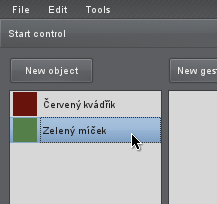
\includegraphics[width=0.5\textwidth]{object.png}
\caption{Zobrazení objektu v hlavním okně}
\end{figure}

Pro úpravu objektu klikněte dvakrát na jeho zobrazení v hlavním okně. Tím
otevřete stejný dialog jako při přidávání objektu a úprava objektu probíhá
také stějně jako přidávání.

Jediné co se v dialogu objeví navíc je tlačítko
\emph{Delete}, kterým můžete objekt smazat. Pokud máte při odstraňování k
objektu přidána nějaká gesta (viz dále), bude Vás aplikace varovat, že dojde i
k jejich smazání.

\subsection{Práce s gesty}
Pro práci s gesty slouží prostřední část hlavního okna. Pro přidání nového
gesta klikněte na tlačítko \emph{New gesture}. Vyjede menu, kde si vybere
jaké gesto chcete přidat. Jsou na výběr tři typy gest -- stavové, vztahové a
pohybové.

Začneme stavovým gestem. Dialog nového stavového gesta umožňuje nastavit
podmínku, kterou musí splňovat vlastnost objektu.

\begin{figure}[h]
\centering
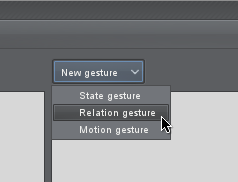
\includegraphics[width=0.5\textwidth]{newgesturemenu.png}
\caption{Menu pro výběr typu gesta pro přidání}
\end{figure}
